\chapter{Wave Motion}

\begin{definition}
    \vocab{Wave motion} refers to the transfer of energy by propagation of oscillations without net movement of the medium.
\end{definition}

Propagation of oscillations in physical media (e.g. air, water) are called mechanical waves. Propagation of oscillations in electromagnetic fields are called electromagnetic waves.

\begin{definition}
    A \vocab{wavelength} ($\l$) is the minimum distance between any two points of the wave with the same phase at the same instant.
\end{definition}

The SI unit of wavelength is the metre (m).

\begin{definition}
    The \vocab{wave speed} ($v$) is the speed with which energy is transmitted by a wave.
\end{definition}

The SI unit of wave speed is metre per second (m s$^{-1}$).

\begin{proposition}
    The wave speed $v$ is related to the wavelength $\l$ and frequency $f$ by \[v = f\l.\]
\end{proposition}
\begin{proof}
    By definition, \[v = \frac{\text{distance travelled in 1 oscillation}}{\text{time taken for 1 oscillation}} = \frac{\l}{T} = f\l.\]
\end{proof}

\begin{definition}
    A \vocab{wave font} is an imaginary line or surface joining points which are in phase.
\end{definition}

Wave fronts are usually drawn one wavelength apart and are often thought to represent wave crests. All the points on a wave front have the same distance from the source of the wave.

\begin{definition}
    A \vocab{ray} is the direction in which the energy of a wave is travelling.
\end{definition}

Rays are always perpendicular to wave fronts.

\begin{definition}
    The \vocab{phase difference} ($\D \f$) between two waves at a point or between 2 points on a wave is the difference in the phases of their oscillation cycle expressed as an angle, where $2\pi$ represents one cycle.
\end{definition}

The phase difference between two waves of the same frequency at a point is equivalent to the time difference for the waves to be at the same oscillation phase, expressed as an angle, where $2\pi$ represents one period. \[\D \f = \frac{\D t}{T} \cdot 2\pi.\]

The phase difference between two points on a wave is equivalent to the distance between the points expressed as an angle, where $2\pi$ represents one wavelength. \[\D f = \frac{\D x}{\l} \cdot 2\pi.\]

\section{Progressive Waves}

\begin{definition}
    A \vocab{progressive wave} is a wave in which energy is carried by means of vibration or oscillation within the waves, without transporting matter.
\end{definition}

Progressive waves can be further classified as either transverse of longitudinal.

\begin{definition}
    A \vocab{transverse wave} is a wave whose vibrations are perpendicular to the direction of transfer of energy of the wave.
\end{definition}

\begin{definition}
    A \vocab{longitudinal wave} is a wave whose vibrations are parallel to the direction of transfer of energy of the wave.
\end{definition}

All electromagnetic waves are transverse.

\begin{definition}
    The \vocab{intensity} ($I$) of a wave is the rate of energy transmitted per unit area perpendicular to the wave propagation.
\end{definition}

The SI unit of intensity is watt per square metre (W m$^{-2}$).

\begin{proposition}
    For a fixed frequency $f$, the intensity $I$ of a wave is proportional to the square of its amplitude $A$.
\end{proposition}
\begin{proof}
    Recall from simple harmonic motion that the total energy associated with an oscillation is given by \[E = \frac12 m \o^2 A^2 = \frac12 m \bp{2\pi f}^2 A^2 = \underbrace{\bp{2\pi^2 m f^2}}_{\text{constant}} A^2.\] Since $I \propto E$ and $E \propto A^2$ (for constant $f$), so $I \propto A^2$.
\end{proof}

\begin{proposition}
    In 3D, the intensity $I$ at a point located a distance $r$ from a point source which emits energy with power $P$ is given by \[I = \frac{P}{4\pi r^2}.\]
\end{proposition}
\begin{proof}
    The area of all points a distance $r$ away from the point source is $4\pi r^2$. Hence, by the definition of $I$, \[I = \frac{\text{energy} / \text{time}}{\text{area}} = \frac{\text{power}}{\text{area}} = \frac{P}{4\pi r^2}.\]
\end{proof}

In 2D, we have the analogous result:

\begin{proposition}
    In 2D, the intensity\footnotemark $I$ at a point located a distance $r$ from a point source which emits energy with power $P$ is given by \[I = \frac{P}{2\pi r}.\]
\end{proposition}
\footnotetext{Note that in 2D, we modify the definition of intensity to ``rate of energy transmitted per unit length perpendicular to the wave propagation.''}

\section{Polarization}

A transverse wave could have a mixture of oscillations in an infinite number of directions, in the plane normal to the direction of energy transfer. This is known as an \vocab{unpolarized wave}.

\begin{definition}
    \vocab{Polarization} is the process by which a wave's oscillations are made to occur in one direction only, in the plane normal to the direction of energy transfer.
\end{definition}

Polarization is a phenomenon associated only with transverse waves (e.g. light). This is because in longitudinal waves, the medium only oscillates in one direction (parallel to the direction of energy transfer).

\begin{proposition}
    The final intensity $I$ of an unpolarized light wave (of initial intensity $I_0$) after passing through a polarizer is given by \[I = \frac12 I_0.\]
\end{proposition}
\begin{proof}
    The unpolarized light wave is a random mixture of all states of polarization, and the vertical and horizontal components are, on average, equal. Hence, the polarizer should transmit 50\% of all incident light, i.e. \[I = \frac12 I_0.\]
\end{proof}

\begin{figure}[H]
    \centering
    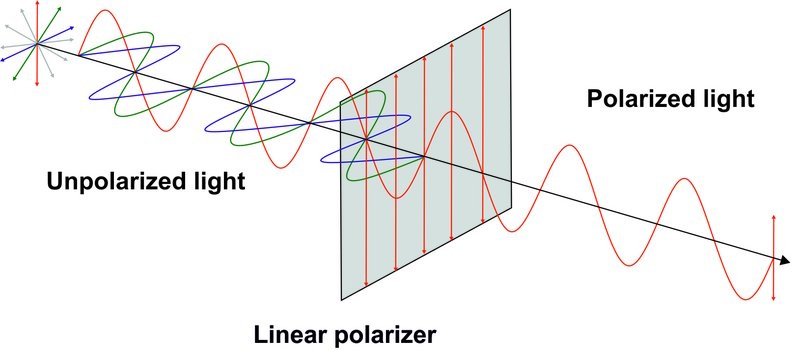
\includegraphics[scale=1.2]{media/Polarizer.jpg}
    \caption{Effect of a polarizer on unpolarized light.\protect\footnotemark}
\end{figure}
\footnotetext{Source: \url{https://www.codixx.com/knowledge-corner/polarization}}

\begin{theorem}[Malus' Law]
    When a polarizer is placed in a polarized beam of light, the intensity $I$ of the light that passes through is given by \[I = I_0 \cos^2 \t,\] where $I_0$ is the initial intensity and $\t$ is the angle between the light's initial polarization direction and the axis of the polarizer.
\end{theorem}
\begin{proof}
    Let $A$ be the initial amplitude of the polarized light wave. When the light passes through the new polarizer, only the components that are parallel to the new polarization direction passes through. The resulting amplitude is thus $A \cos \t$. Since intensity is proportional to amplitude squared, we have \[I = k\bp{A \cos \t}^2 \quad \tand \quad I_0 = kA^2\] for the same constant of proportionality $k$, so \[\frac{I}{I_0} = \cos^2 \t \implies I = I_0 \cos^2 \t.\]
\end{proof}